\chapter{Leveraging Time vs Space Division Multiplexing}\label{ch:leveraging-time-division-multiplexing}

When a chunk of data is available at a given time for processing, it can all be processed at the same time, or pieces after pieces.
Processing simultaneously all the data offers the advantage of a reduced latency, but requires creating copies of the processing 
blocks for each piece. A sequential processing gives the possibility of having just one processing block treating the data step 
by step at a price of latency.

A simple parallel with human body is our hands. When writing a text, because of our small number of hands we are condemned to write 
texts one letter after another. But if we imagined having 1000 hands, and enough space to hold as many pen without interfering with one another,
we could imagine writing whole paragraphs at once.


\section{Time Division Multiplexing}\label{sec:time-division-multiplexing}
The time division multiplexing approach consists in sharing the resources, or processing blocks, by routing each piece of data depending on time \(t\). Choosing this implementation can be intuitive as computers usually process data using frames of 32 to 64 bits. It has the advantage of reusing design blocks hence possibly reducing area usage, but performs poorly in case of data dependencies. If the word from time \(t=0\) of the frame needs to be available at the same time as the one of \(t=4\), the logic becomes very complex thus canceling the positive area impact unlocked by resource sharing.

This sequential processing approach requires counters used by multiplexers to latch the input data at the right moments. This approach is represented in figure \ref{fig:time-division-multiplexing}.

\begin{figure}
    \begin{subfigure}[c]{.5\textwidth}
        \centering
        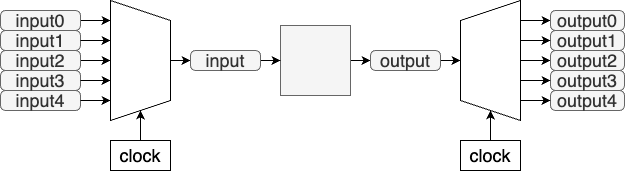
\includegraphics[width=1\linewidth]{tdm.png}
        \caption{Block Diagram}
    \end{subfigure}
    \begin{subfigure}[c]{.5\textwidth}
        \centering
        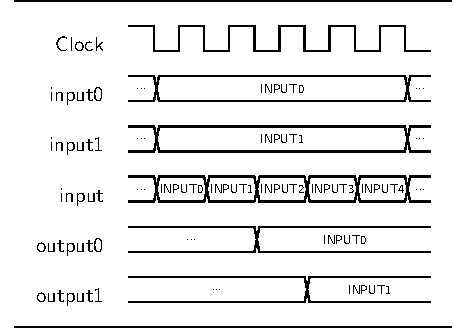
\includegraphics[width=1\linewidth]{../timings/tdm.pdf}
        \caption{Timing}
    \end{subfigure}
    \caption{Time Division Multiplexing}
    \label{fig:time-division-multiplexing}
\end{figure}

\section{Space Division Multiplexing}
Another way of treating the data is to make it all available at the same time, as parallel inputs of the processing block. This approach is more natural as it is closer to what humans experience; we see, hear, feel, taste at the same time, not one after the other. It is represented in figure \ref{fig:space-division-multiplexing}. Space Division Multiplexing generally offers small latencies, as every block runs in parallel and reduces the use of sequential logic which would be required in TDM. In fact, using a parallel logic, some processing blocks can become purely combinational ones.

\begin{figure}
    \begin{subfigure}{.5\textwidth}
        \centering
        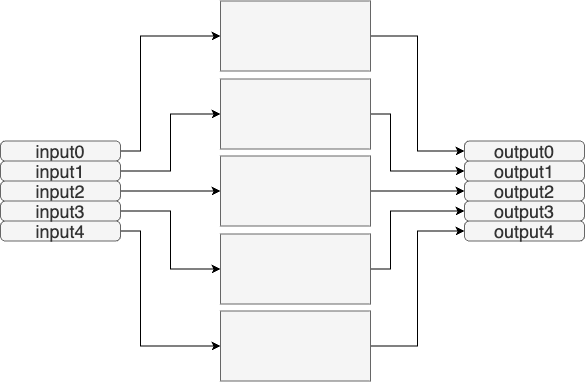
\includegraphics[width=1\linewidth]{sdm.png}
        \caption{Block Diagram}
    \end{subfigure}
    \begin{subfigure}{.5\textwidth}
        \centering
        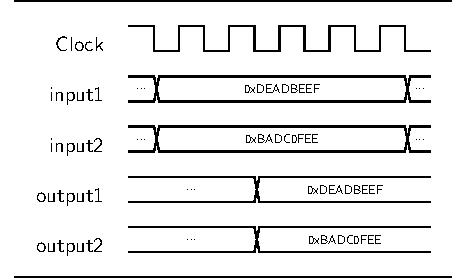
\includegraphics[width=1\linewidth]{../timings/sdm.pdf}
        \caption{Timing}
    \end{subfigure}
    \caption{Space Division Multiplexing}
    \label{fig:space-division-multiplexing}
\end{figure}

\section{Tradeoffs}\label{sec:space-versus-time-division-multiplexing}
Whether one approach is better than the other is impossible to determine prior to having a deep understanding of the data processing blocks.
The most common tradeoff is the one of latency at the price of area. But the Maximal Operating Frequency (\(F_{max}\)) can also be traded to 
improve other metrics.

Having access to all variables at the same time makes the code development easier.


\section{Leveraging Both Approaches for LATOME}
In the version 6 firmware the choice was made to use parallel data as much as possible as it showed promising preliminary results. The input and output interfaces of both ISM and OSUM are indeed fully parallel.

\begin{figure}
    \centering
    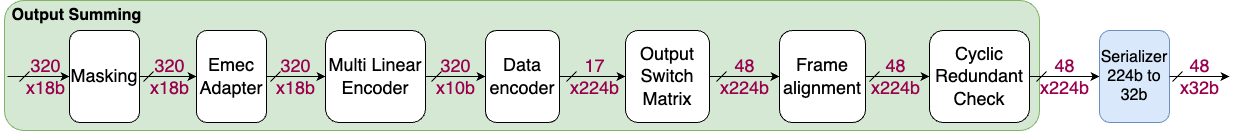
\includegraphics[width=1\textwidth]{osum_v6.png}
    \caption{Output Summing Block Diagram}
    \label{fig:osum-v6}
\end{figure}

The Output Summing represented in figure \ref{fig:osum-v6} is made of the following blocks:
\begin{itemize}
    \item Masking: responsible for disabling some inputs depending on the detector region that a specific LATOME treats
    \item Emec Adapter: this block performs additional summing for the LATOME responsible for the EMEC region of the detector
    \item Multi Linear Encoder (MLE): Since the ADC readings are 12 bits long but the FEX systems requires 10 bits long energy levels, this block encodes the ADC readings on 10 bits
    \item Data Encoder: Once the encoded energy levels are ready, this block creates 17 frames of 224 bits representing the whole data
    \item Output Switch Matrix (OSM): This switch matrix routes the 17 224 bits frames to the different FEX systems that the LATOME is connected too
    \item Frame Alignment: Each couple of BC, the LATOME does not send any data but instead it sends an alignment frame built by this block
    \item CRC9: This final block appends to the last 9 bits of each frame a CRC9 value which it computes
\end{itemize}

The OSM, which is further described in Section \ref{sec:osm}, takes large inputs of 224 bits. When working with such data widths, different points of optimization arise. The data synchronization becomes much more complex as 224 signals simultaneous signals must be processed. Consequently, such implementations can block the \(F_{max}\) to low values. 
Then, the OSM uses multiplexers to route the data to the FEX systems. These can become very big with multiple inputs each of 224 bits hence yielding high area usages.

The OSM is a good candidate to use TDM and process smaller pieces of data sequentially.
